\documentclass[a4paper,10pt,fleqn]{jsarticle}
\usepackage{amsmath}
\usepackage[dvipdfmx]{graphicx}


\title{プロジェクト実習テーマP CloudBM  中間レポート2}
\author{
  チームF \\
  C0114312 高畑 達也\\
  C0114015 新井 幸希\\
  C0114234 後藤 尚輝\\
  C0114088 上原 安里奈\\
}
\date{\today}


\begin{document}
\maketitle

\section{システム概要(新井)}
現状ブラウザのブックマークシステムのUIは非常に貧弱であり,デフォルトの状態で大量に存在するブックマークを整理する際,多くの工数がかかってしまう.
 この乱雑に増え続けるブックマークに対する効果的なアプローチは現在存在せず,ブックマークサービスとして現存するSpeed DialやBookmark Managerのようなアドオンを使うことである程度の整理することができるが,大量のブックマーク整理に向いていない.
 上記の問題を解決するべく,我々はシンプルにブックマークを管理するCloudBMを作成した.CloudBMを使うことにより,たった数回の操作で簡単に大量のブックマークを整理することが可能となる.具体的にはフォルダ分けやタグ付けを行い,さらにリンク切れをしたブックマークの削除などを自動で行い,ユーザーはただまとめられたブックマークを検索をすれば良い.
\subsection{実装した機能}
\begin{itemize}
\item ブックマークの表示
\item ブックマークの操作
\begin{itemize}
\item DnDによるブックマークのフォルダ移動
\item DnDによるブックマークの並び替え
\end{itemize}
\item ブックマークの検索とグルーピング
\begin{itemize}
\item タイトル等からの検索
\item ブックマークのページ内容による検索
\end{itemize}
\end{itemize}

\subsection{システム構成}
以下に本システムのシステム構成を示す.
\begin{figure}[htbp]
  \begin{center}
    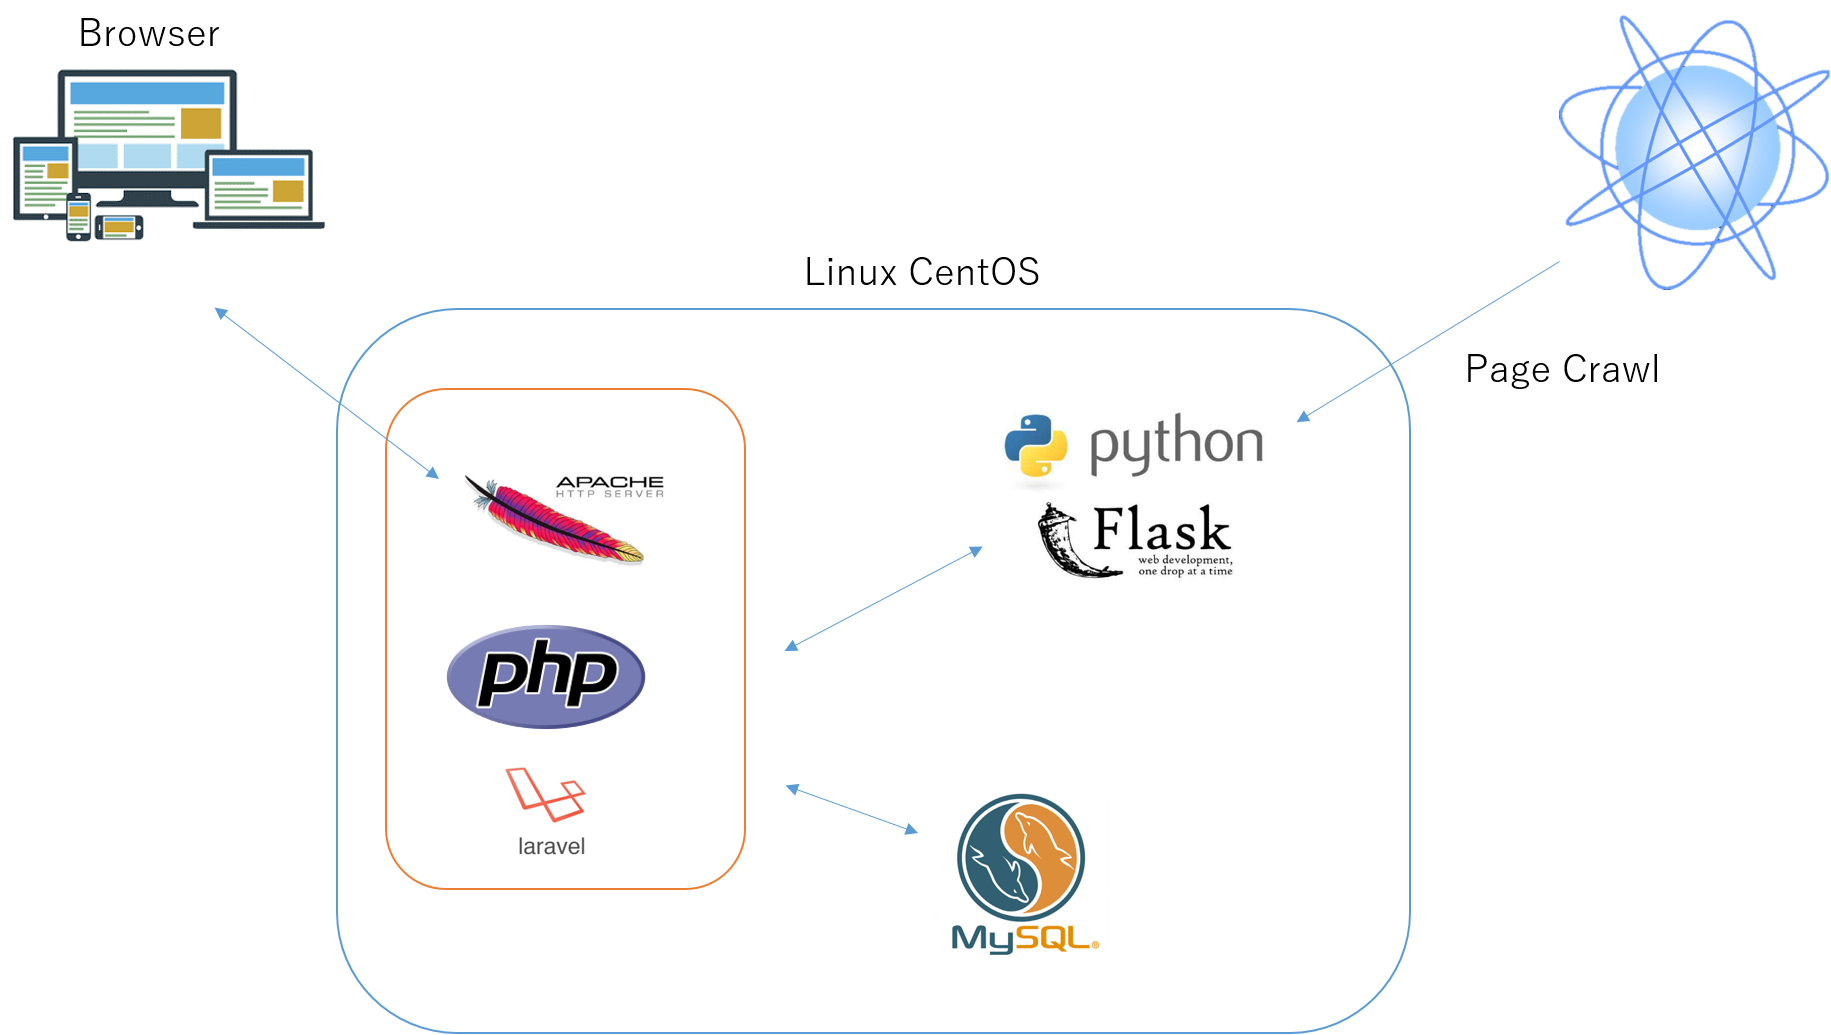
\includegraphics[clip,width=7.0cm]{./architecture.png}
    \caption{システムアーキテクチャ}
    \label{fig:system}
  \end{center}
\end{figure}
本システムはSPAとして構成する.\par
図にしめしたように,フロントサイドではJSフレームワークとしてVuejsを用いる. またサーバーとの通信に関してはAjaxを利用する.
サーバーサイドはLinux環境内にWEBサーバーとしてApacheを,データベースとしてMySQLを用意する. ApacheではPHPを利用しフロントサイドより呼び出すAPIを実装する.\par
加えてサーバーサイドではブックマークの内容解析を行うためのAPIを用意する. このAPIはpythonとpythonのWebフレームワークであるflaskで構成されておりphpから利用される.\\
\par
使用する主なソフトウェア・言語・ライブラリのバージョンについては以下の通りとする.
\begin{itemize}
 \item フロントエンド
    \begin{itemize}
    \item HTML5
    \item CSS3
      \item Bootstrap 3.6
      \item ES5
      \item Vuejs 1.x系
     \end{itemize}
 \item サーバサイド
     \begin{itemize}
    \item PHP 7
    \item Laravel  5.1
      \item MySQL 5.6
      \item Python 3.5
      \item Flask 0.11
     \end{itemize}
\end{itemize}
\section{プロトタイプの説明(高畑)}
このサービスに対して,価値があるのかを調査するため,インタビューを行った際にインタビュー対象者へ見てもらうプロトタイプの作成を行った.実際にインタビューを行う過程でプロトタイプを見てもらい,サービスの動きを視覚的に理解してもらうことが目的である.下記の図\ref{fig:prot1}はCloudBMのプロトタイプである.

\begin{figure}[h]
  \begin{center}
    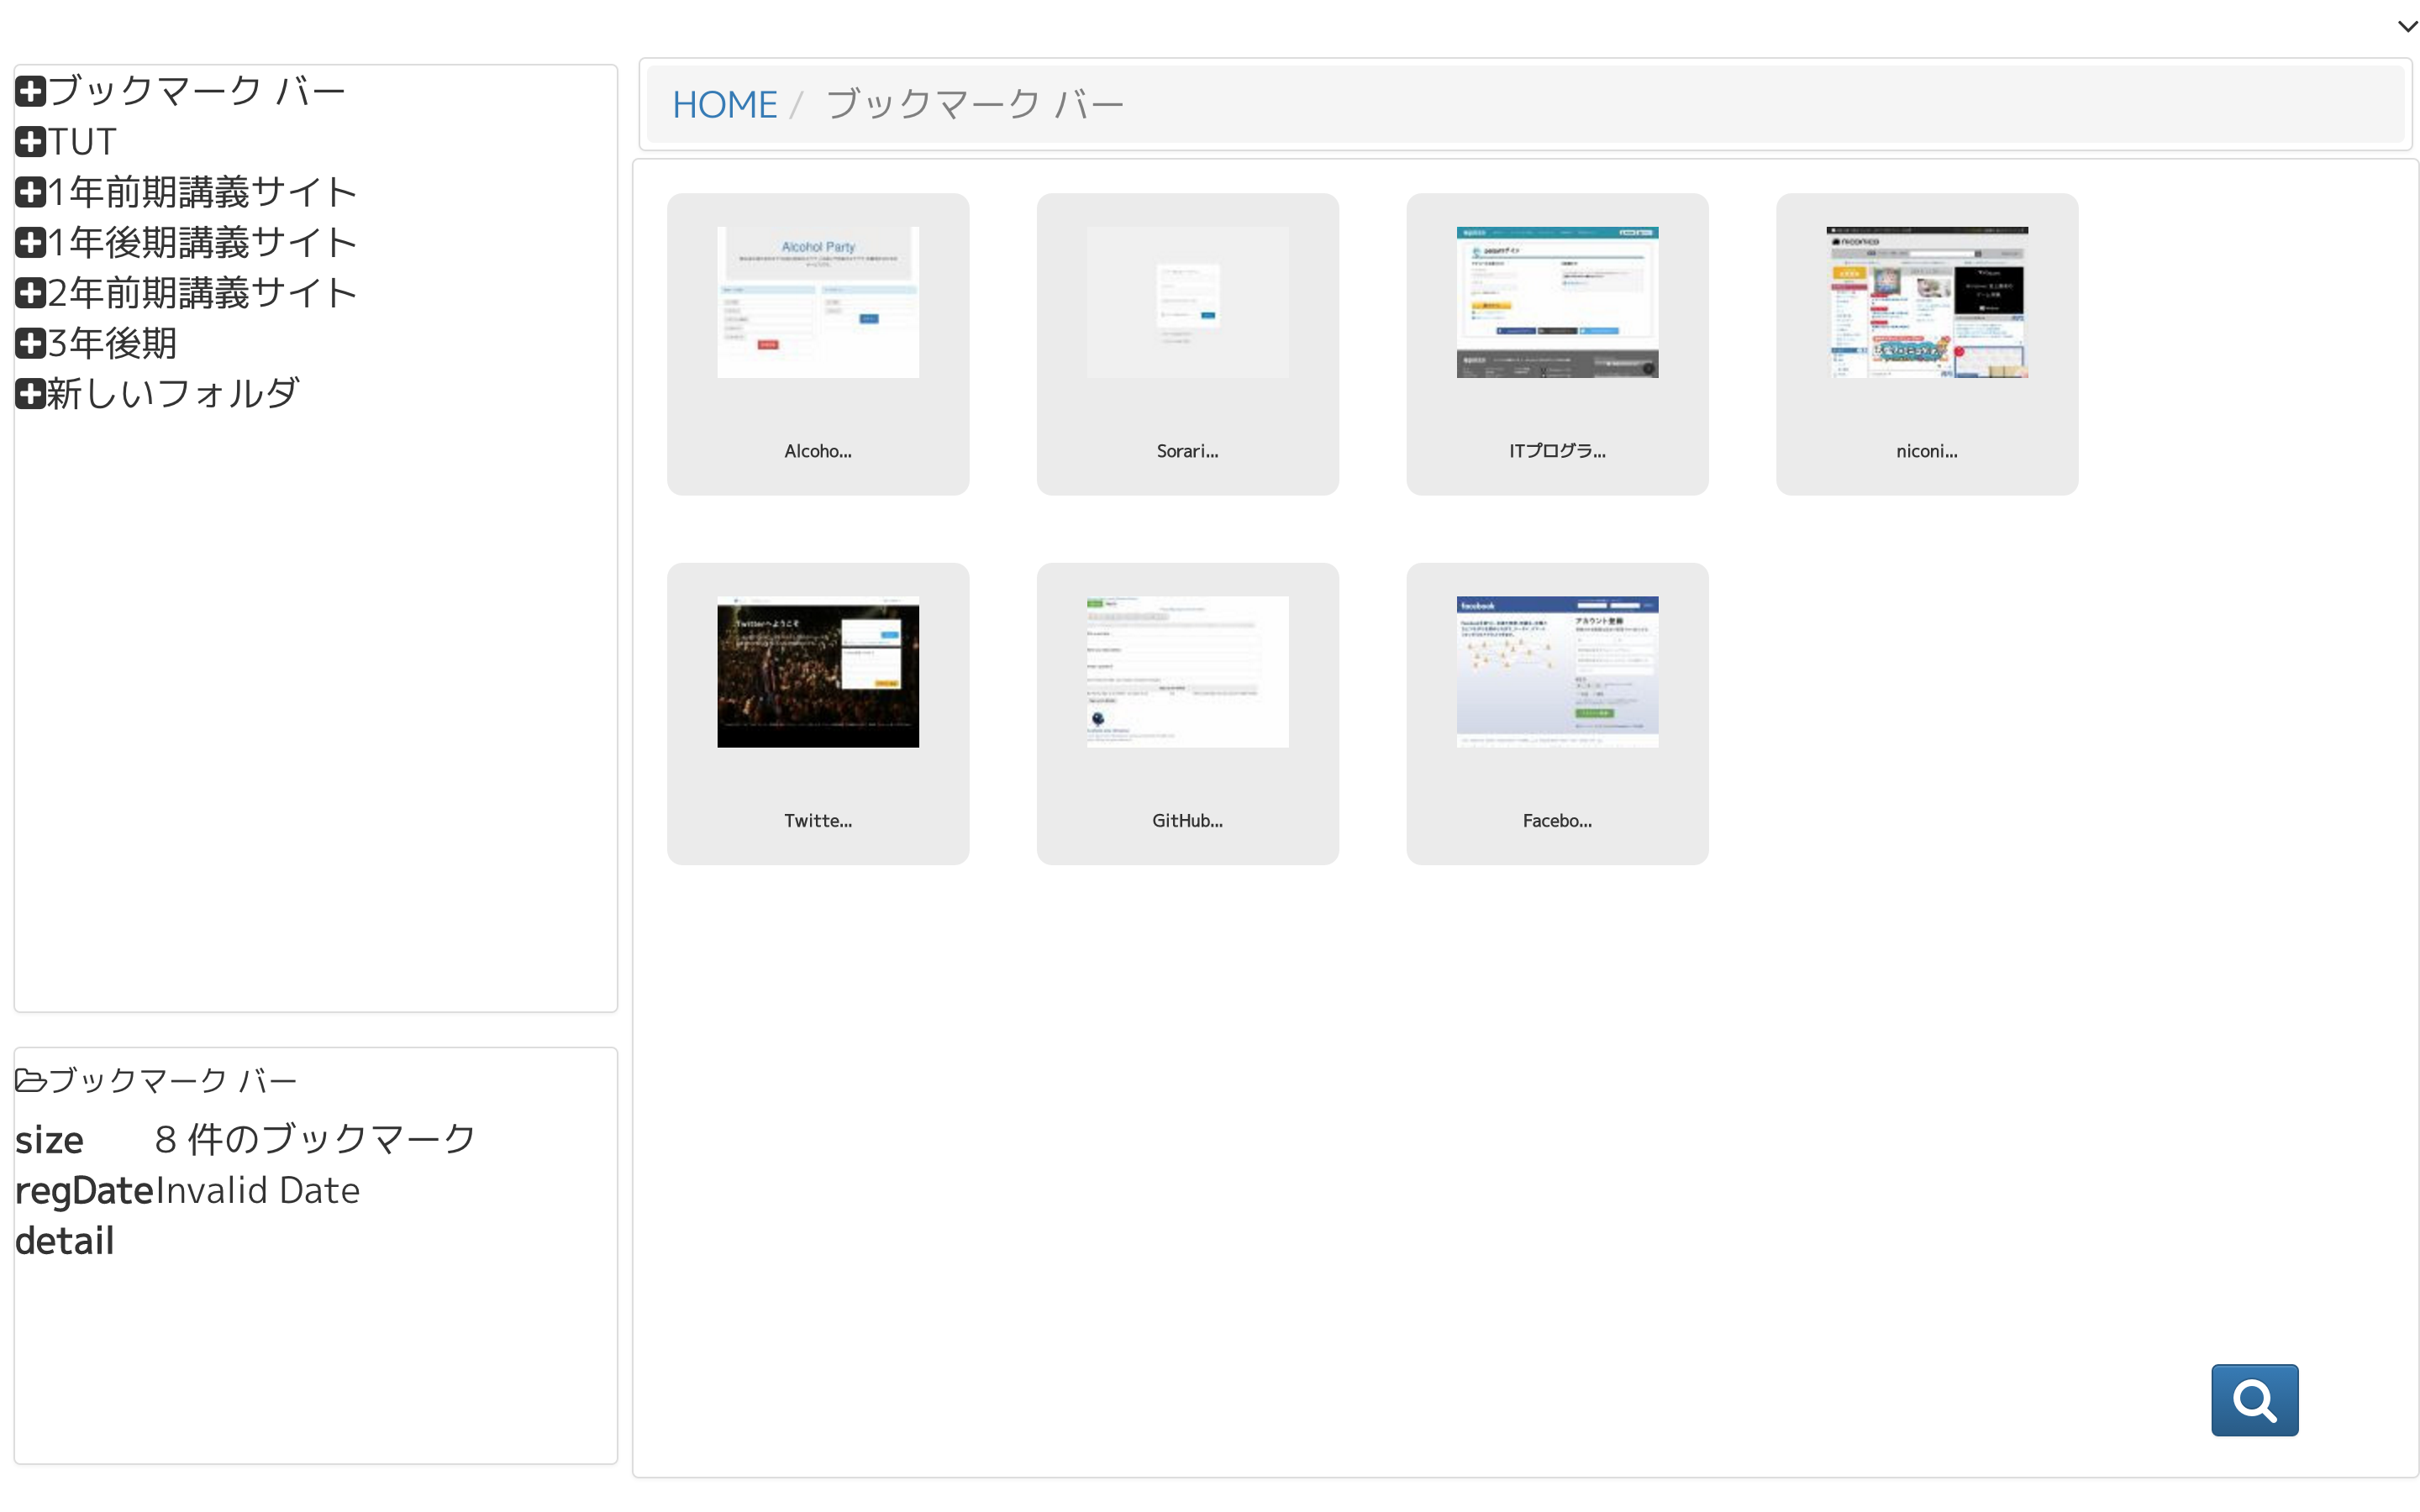
\includegraphics[width=9.0cm]{./prot1.png}
    \caption{プロトタイプ画面}
    \label{fig:prot1}
  \end{center}
\end{figure}

画面左側には,ブックマークフォルダのツリー構造,右側にはフォルダに格納されているブックマークが表示される.現状,動画サイトや各種SNSのページなど,様々なブックマークが表示されていて,整理出来ているとは言い難い.これらのブックマークを整理するため,画面下部の検索マークをクリックしキーワードの検索を行う.動作画面を図\ref{fig:prot2}に示す.

\begin{figure}[h]
  \begin{center}
    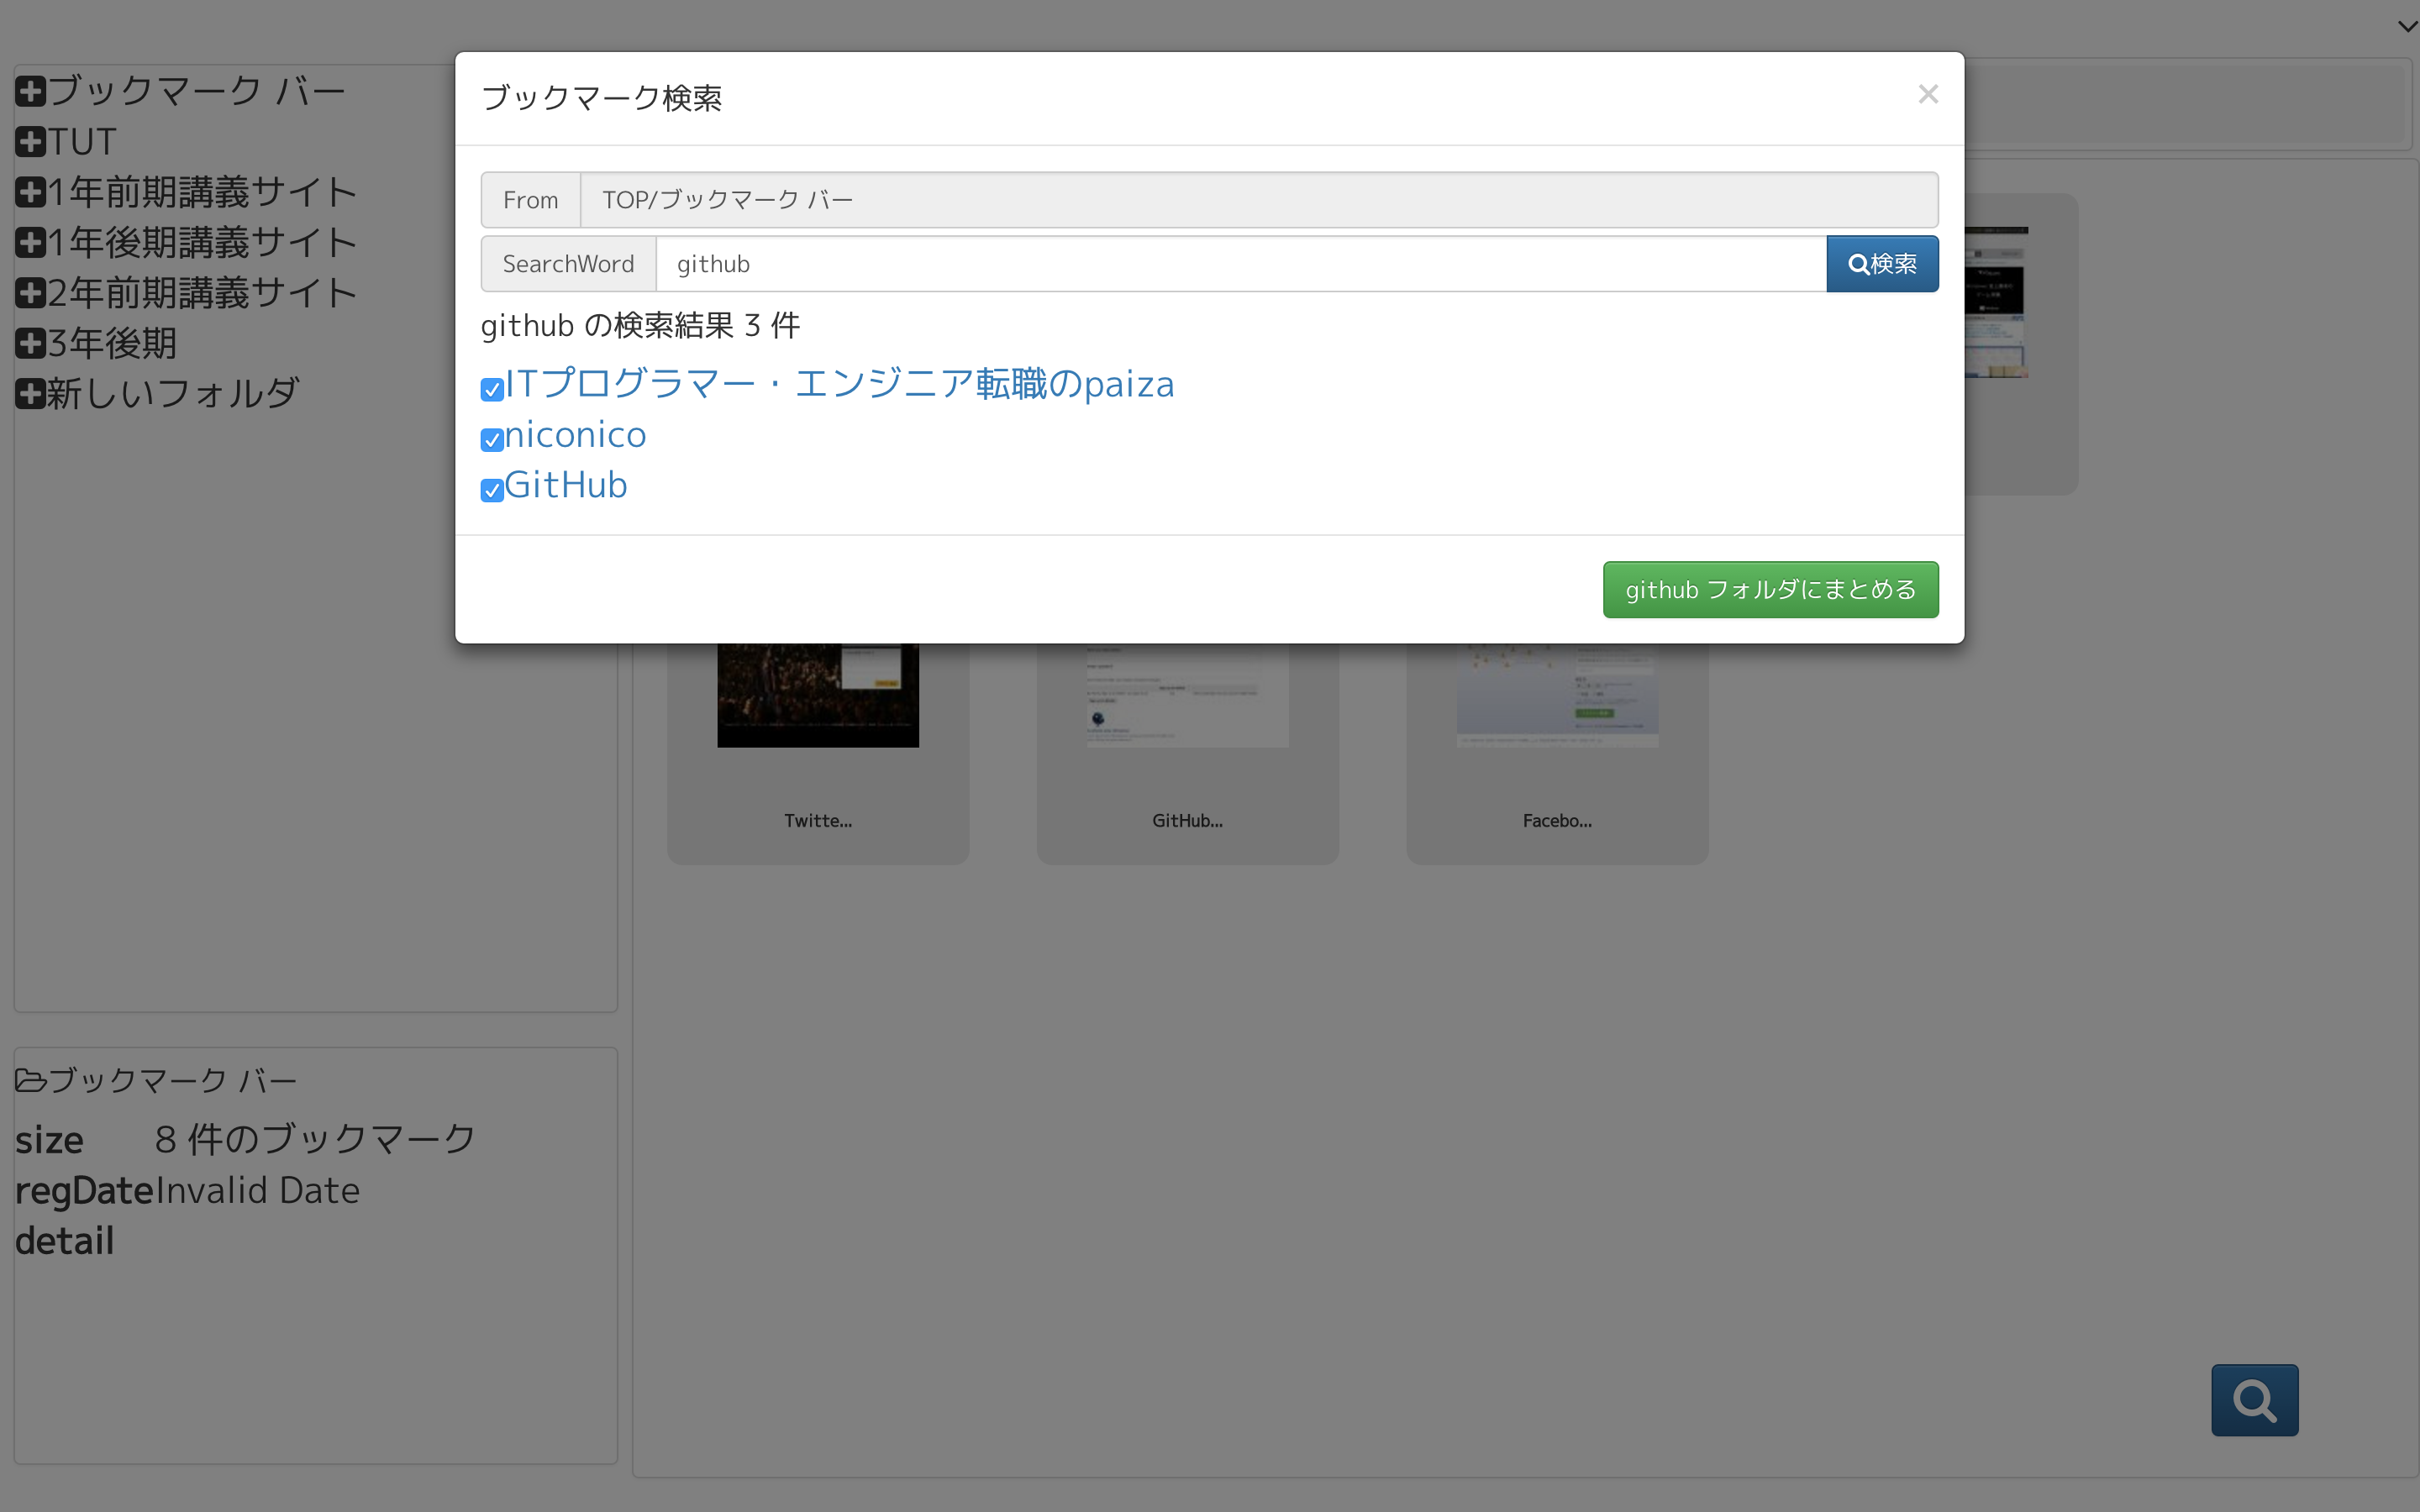
\includegraphics[width=9.0cm]{./prot2.png}
    \caption{キーワード検索画面}
    \label{fig:prot2}
  \end{center}
\end{figure}

テキストボックスにキーワードを入力することで,関連するブックマークの一覧を確認することができ,またフォルダに纏めたい場合にはボタンをクリックするだけで,関連するブックマークを一つのフォルダに簡単に整理することができる.整理した際の画面を図\ref{fig:prot3}に示す.

\begin{figure}[h]
  \begin{center}
    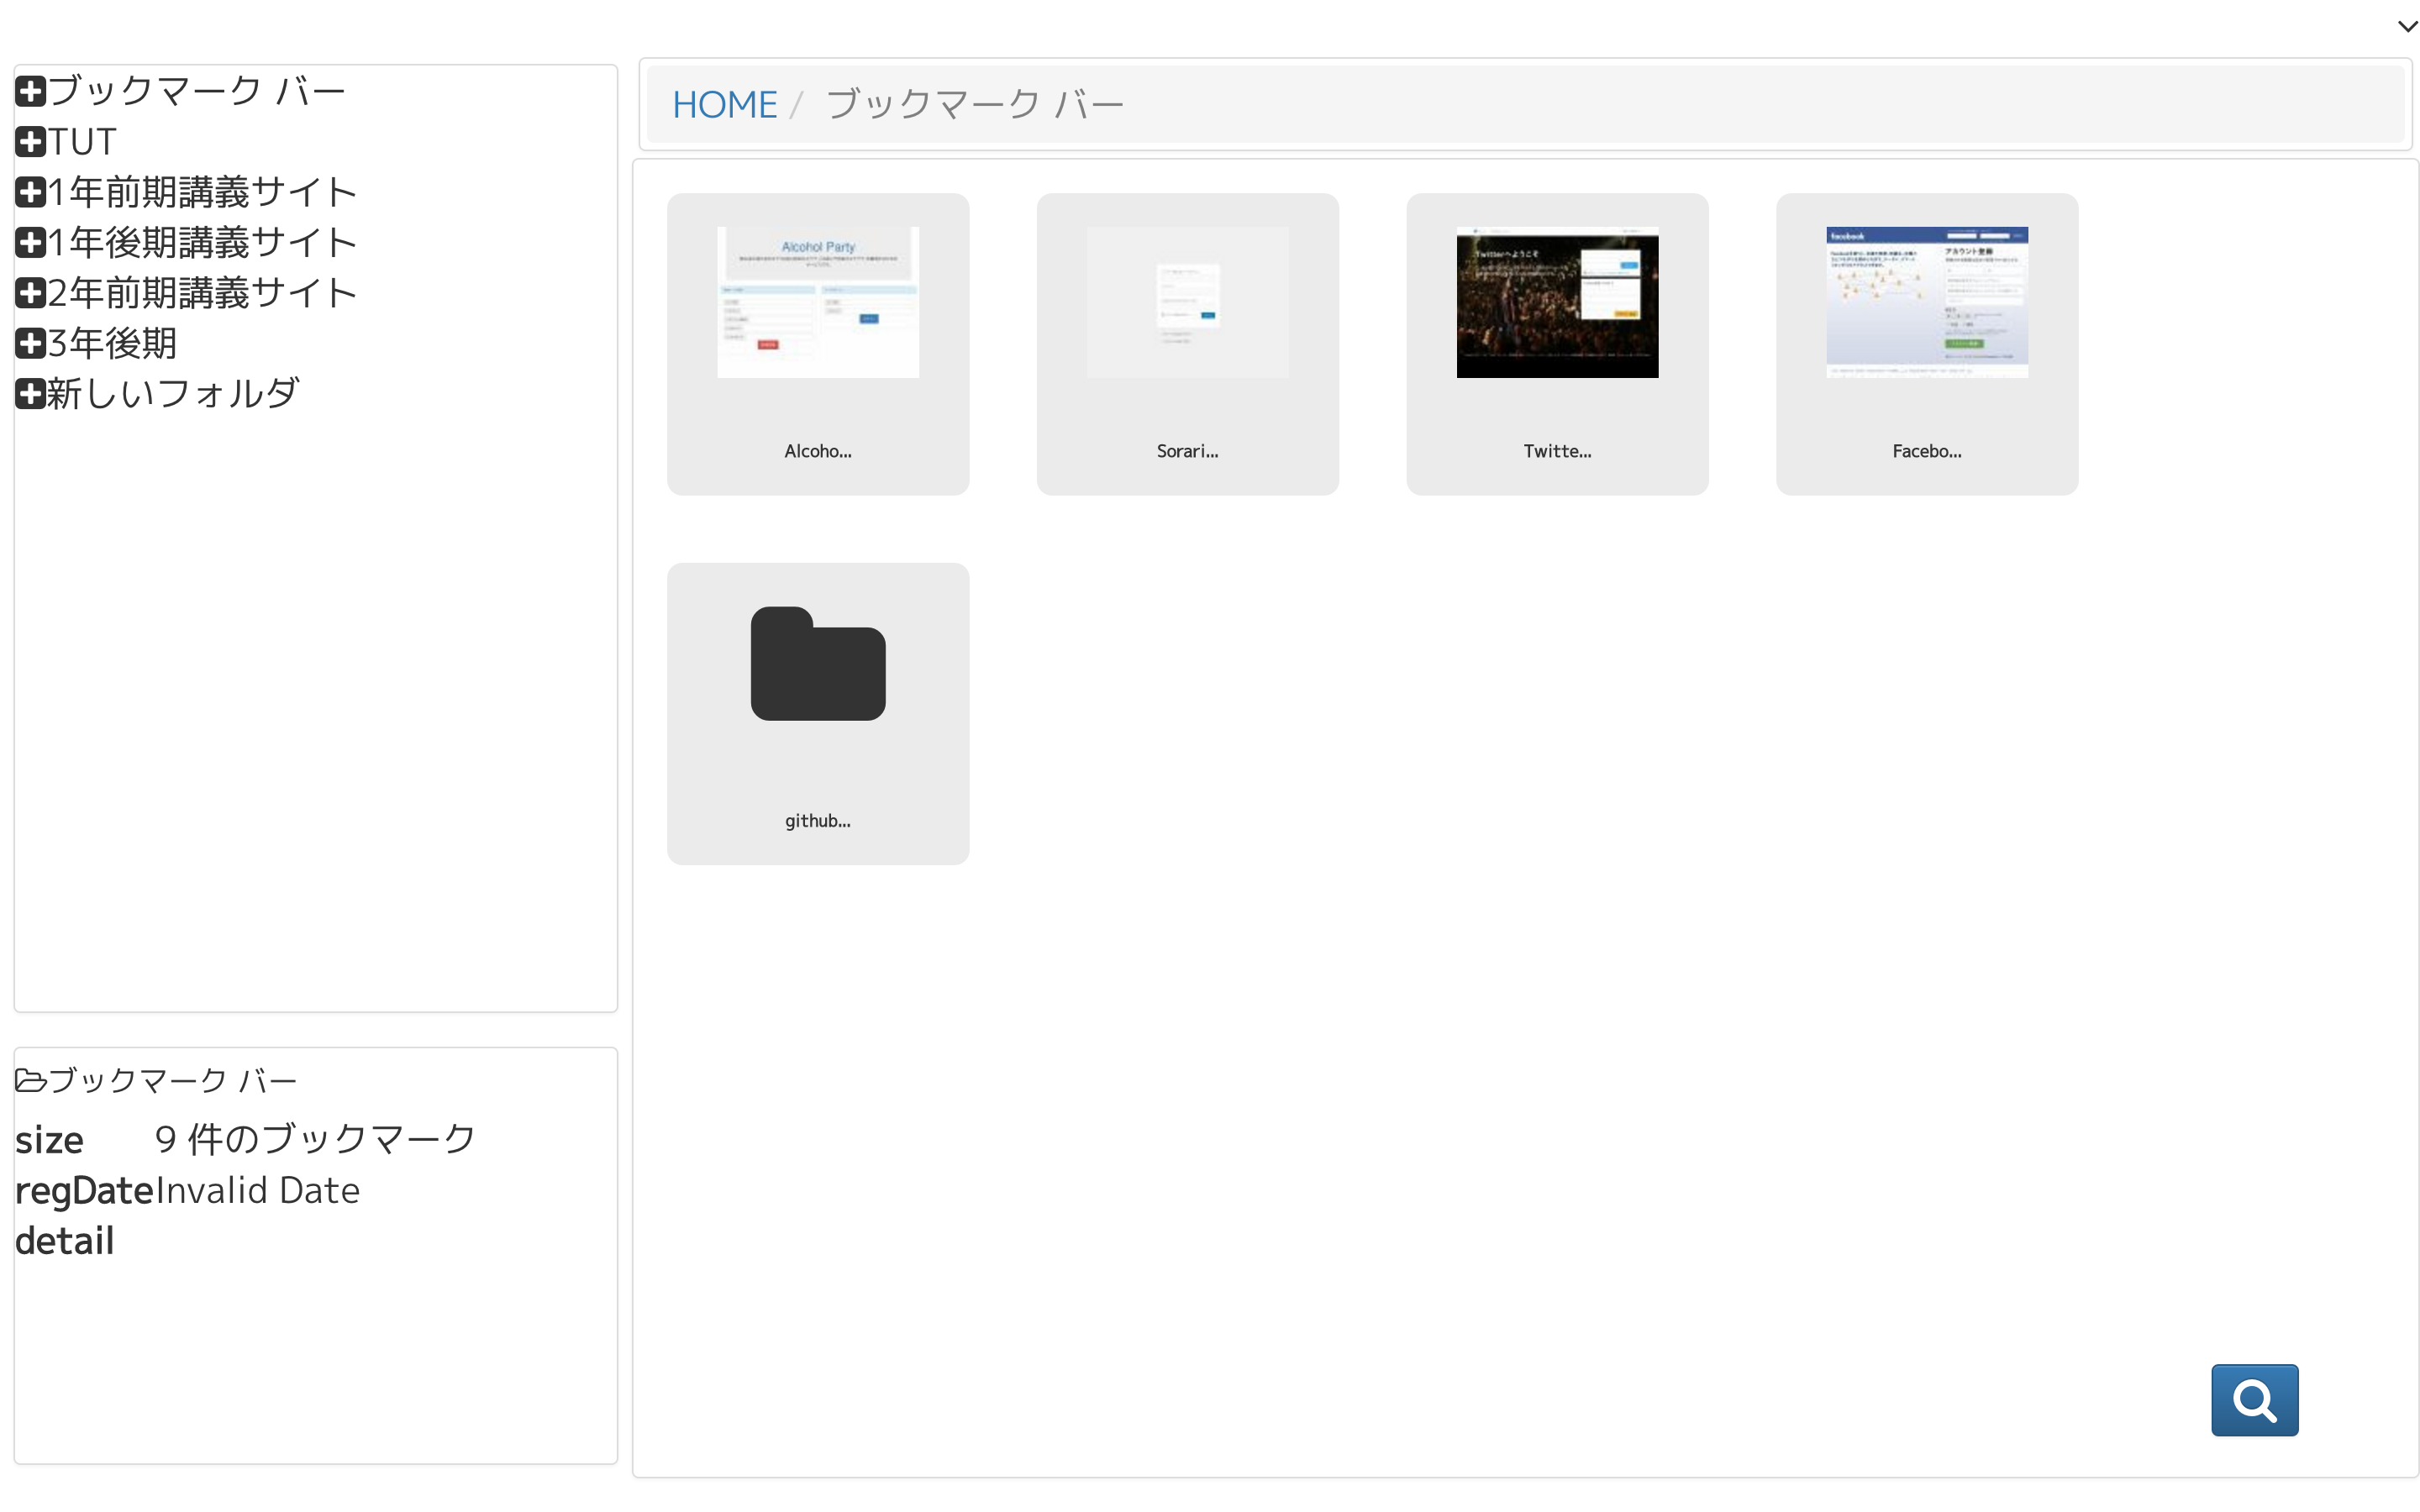
\includegraphics[width=9.0cm]{./prot3.png}
    \caption{フォルダ整理後の画面}
    \label{fig:prot3}
  \end{center}
\end{figure}

\newpage

図\ref{fig:prot3}を見て分かるように,「GitHub」というキーワードに基づくブックマークがフォルダに纏められる.整理が完了したブックマークは,アドオンを利用することにより,Webブラウザと自動同期することが出来る.このシステムを利用することにより,これまで大量に存在したブックマークを手動でフォルダ分けする必要がなくなり,より良いブラウジングが可能となる.

また,ブックマークに登録されているデータは,DnDで移動ができ,よりエクスプローラライクな操作感を実現した.また,不要になったWebページは右クリックで出現するコンテキストメニュー(図\ref{fig:prot4})より,削除をすることが出来る.

そして,付加機能として,ブックマークデータをダブルクリックすることで,即座にWebページを開くことが出来るため,ブックマークを整理するだけではなく,そのままブックマークとして使用することも可能である.

\begin{figure}[h]
  \begin{center}
    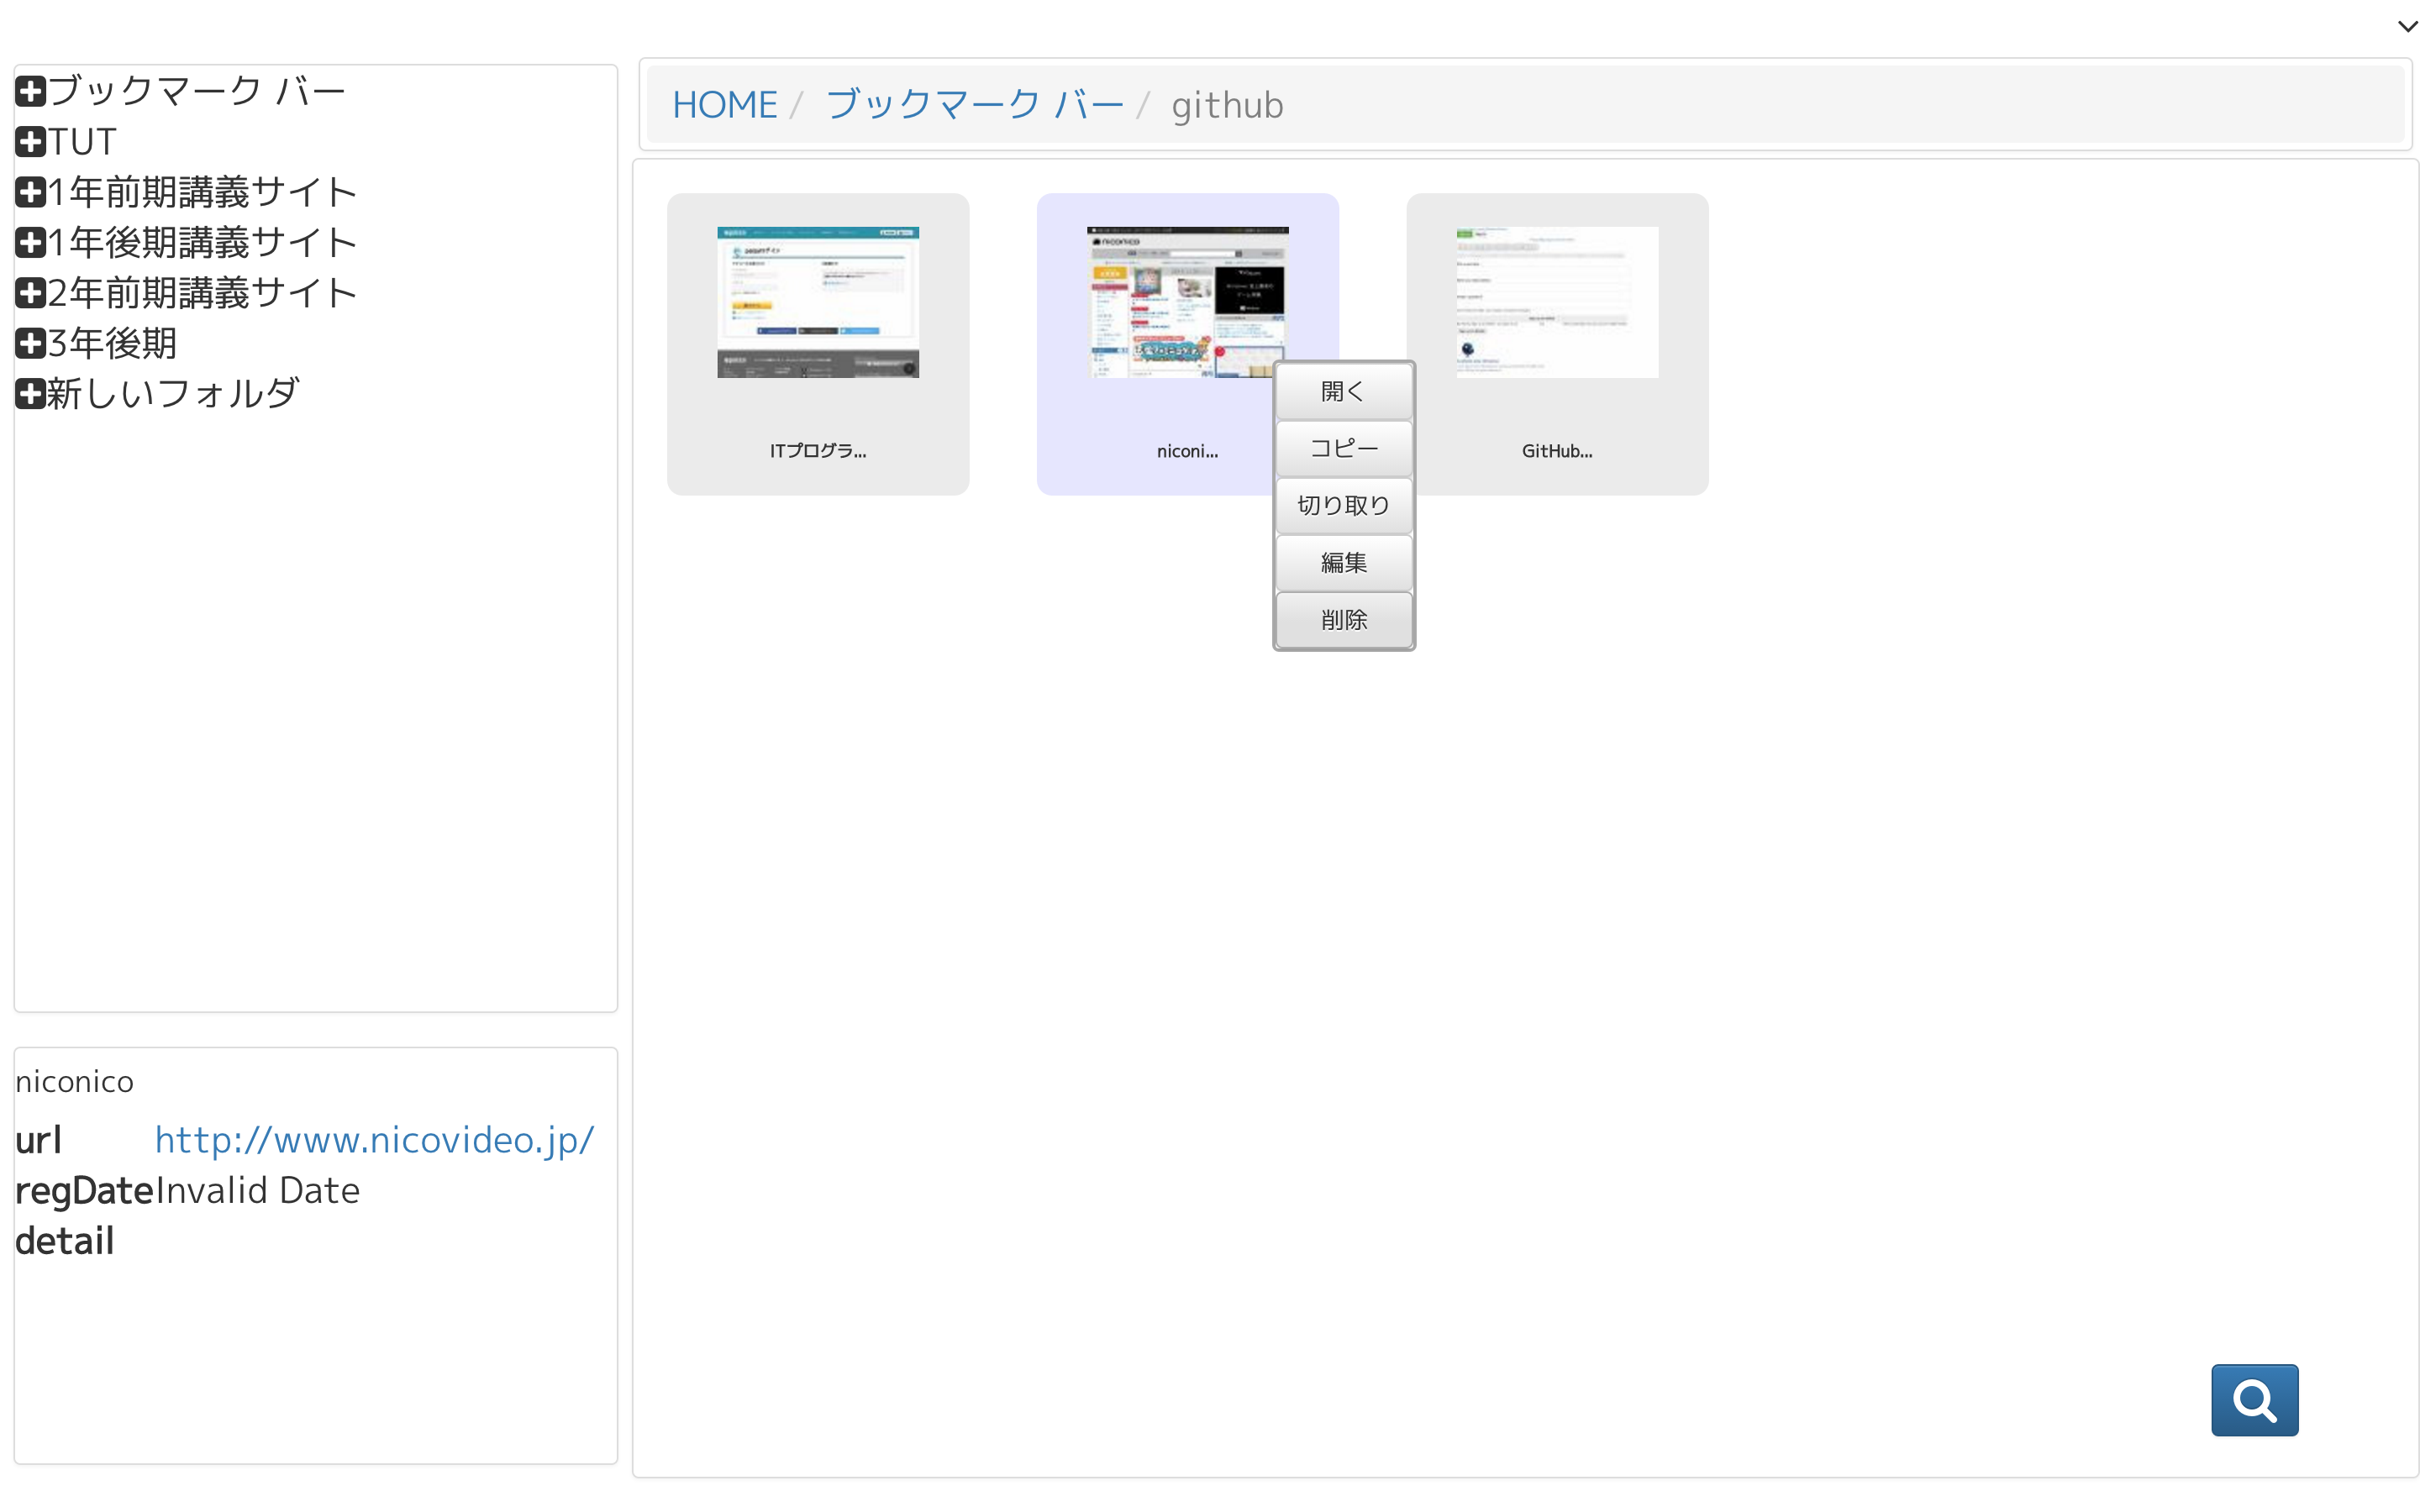
\includegraphics[width=9.0cm]{./prot4.png}
    \caption{コンテキストメニュー}
    \label{fig:prot4}
  \end{center}
\end{figure}

\newpage

\section{顧客インタビューとその解析(上原)}

\subsection{インタビューの目的}
対象ユーザー及びコアユーザーの確認と,現在考えているサービスに価値があるのかという確認をするためにインタビューを実施した.

\subsection{インタビュー人数}
インタビューシートとプロトタイプを用いて,IT関係の人を中心に9人にインタビューを実施した.

\subsection{インタビュー解析}
インタビューを実施した人の中でブックマークの数が100個以上であったのは33\%であった.30個以上の人も合わせると78\%であり,IT関係の人はブックマークが多いと考えられる.また、ブックマークの内容に関しては,技術系ページという回答が目立った.どうブックマークを整理出来たら嬉しいかという質問では「自動分類」という回答が多く,現在のプロトタイプ,サービスに対しては「操作回数の多さ」「自動同期」「自動分類」「タグ付け」などの指摘があった.現在のサービスでは使わないと答えたのが67\%であったため、改善する必要がある.しかし「操作回数の多さ」「自動同期」「自動分類」「タグ付け」など改善が改善されれば使うとの回答が得られた事から,ザービス自体の価値はあり、ターゲットユーザーは存在すると考えられる.

\section{結論(後藤)}
プロトタイプを用いたインタビューの結果や
Googleフォームを用いた市場調査から一定数サービスを利用するユーザーがいることが分かった.
インタビューからは現状のプロトタイプに対する不満が明らかとなったためこれらに対処しサービスの質をこれから高めていく.

\subsection{今後の実装方針}
\subsubsection{フロント}
インタビュー結果から分かるように,現状のUIの完成度は低い.
そのため今後はある程度の機能拡張を図りつつも現状のプロトタイプからUIの完成度を高めていく. UIの完成度を高めるにあたっては自分たち以外にも感想を求めるといったUXテスト手法を用い客観的に使いやすいと言えるUIへと昇華させていく.
\par またブラウザ上の画面だけではなくアドオンを提供し解決を図ることが効果的な課題がインタビューから明らかになった. よって今後はページだけではなくブックマークアドオンも作成していくこととする.
\par 作成するアドオンについてはGoogleChromeアドオンとし,機能については
\begin{itemize}
  \item ブラウザブックマークと本サービスのブックマーク同期
  \item ブックマーク追加時に機械学習に基づいたフォルダ分けのサジェスト
  \item ブックマークへのページ内容のタグ付け
\end{itemize}
これらを中心に実装する. 実装時間が取れる場合は機能拡充及びChorome以外のブラウザのアドオン(Firefox等)も開発していく.

\subsubsection{サーバサイド}
現状フロントはモックのみで動作しているためサーバサイドとブックマークデータのやり取りが行えるように連結させていく.随時モックを実装クラスへと置き換え動作するものとしていく.
\par 機械学習を用いたページ内容の分析は現状非常に処理時間がかかる等の問題がある. アルゴリズムの改良やデータのキャッシング,DBに上がったブックマークデータを事前解析する等の工夫を施し処理時間の改善を行っていく.また検索精度は良いとお世辞にも言えない状態であるためアルゴリズムの改良を行っていく.

\subsection{今後の調査方針}
プロトタイプを改良しUI等について調査し改良していく事に加え,
サービスの料金等についてあまり深く考えられていない現状であるので,この金額で出したらサービス使う人がいるかといった事を調査していく.

\section{質問内容とインタビュー結果(後藤)}
インタビューは以下のように行った. またインタビューはできるかぎりコアユーザーにマッチするITエンジニアを対象に行った.
\begin{enumerate}
  \item 対象ユーザであるか判断する質問
  \item サービスの説明をし実際にプロトタイプを触ってもらう
  \item サービスに対する感想を求める
\end{enumerate}

\subsection{質問内容}
実際の質問内容は以下の通りである
\begin{enumerate}
  \item 対象ユーザーであるか確認する質問
  \begin{enumerate}
    \item 何をしている人か
    \item ブックマークはいくつくらいあるか
    \item ブックマークで困っていること 不満があるか
    \item 何をブックマークしているか
    \item ブックマークを整理しているか(その理由,整理する既存サービスを利用しているか)
    \item どのようにブックマークが整理できたらうれしいか
  \end{enumerate}
  \item サービスに関する質問
  \begin{enumerate}
    \item どんなサービスだと思ったか(伝わったか)
    \item このサービスを利用するか
    \item このサービスについてどう思うか(使うか)
    \begin{enumerate}
      \item 操作の回数
      \item UI
      \item 操作性
    \end{enumerate}
    \item (サービス使わないと答えた場合)この内容が改善されたら利用するか
  \end{enumerate}
\end{enumerate}
\subsection{インタビュー結果}
質問に関する回答結果は以下のようになった

\begin{figure}[htbp]
  \begin{center}
    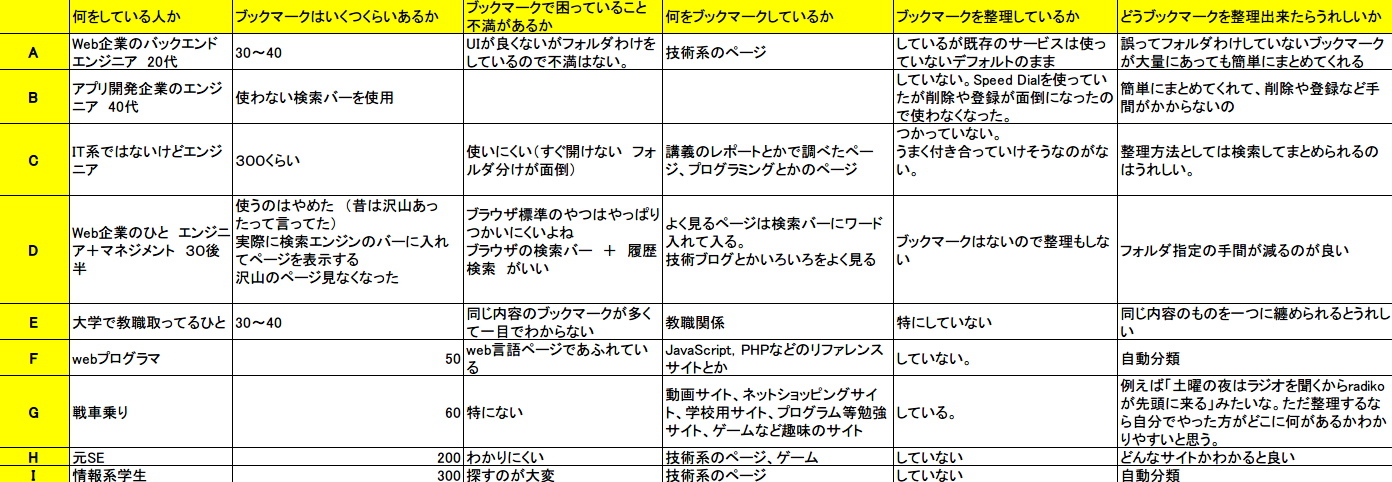
\includegraphics[width=14cm]{./interview-res-1.png}
    \caption{ブックマークに関する質問}
  \end{center}
\end{figure}
\begin{figure}[htbp]
  \begin{center}
    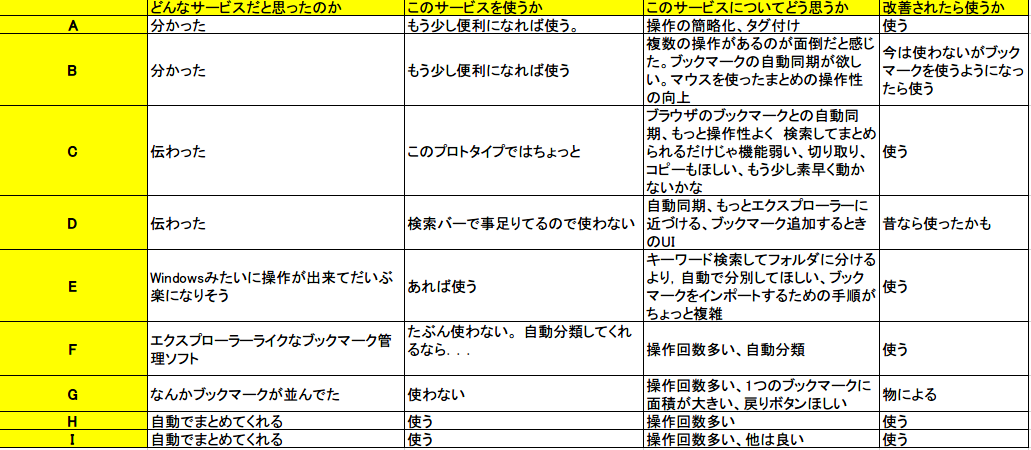
\includegraphics[width=14cm]{./interview-res-2.png}
    \caption{サービスに関する質問}
  \end{center}
\end{figure}


\end{document}
